\documentclass[oneside,openany,headings=optiontotoc,11pt,numbers=noenddot]{scrreprt}

\usepackage[a4paper]{geometry}
\usepackage[utf8]{inputenc}
\usepackage[T1]{fontenc}
\usepackage{lmodern}
\usepackage[ngerman]{babel}
\usepackage{ngerman}

\usepackage[onehalfspacing]{setspace}

\usepackage{fancyhdr}
\usepackage{fancybox}

\usepackage{rotating}
\usepackage{varwidth}

%Struktogramme
\usepackage[german,curves]{struktex}

\usepackage{pdflscape}
\usepackage{changepage}
\usepackage{graphicx}
\usepackage[bottom]{footmisc}
\usepackage{transparent}
\usepackage{graphbox}
\graphicspath{
	{Pics/PDFs/}
	{Pics/JPGs/}
	{Pics/PNGs/}
}
\usepackage{caption}
\usepackage{wrapfig}
\usepackage{marginnote}
\usepackage{tabularx}
\usepackage{dashrule}
\usepackage{soulutf8}
\usepackage{hhline}
%arydshln suppresses vertical lines in table
%\usepackage{arydshln}
\usepackage{multirow}
\usepackage{enumerate}
\usepackage[hidelinks]{hyperref}
\usepackage{listings}

\usepackage[table]{xcolor}
\usepackage{array}
\usepackage{enumitem,amssymb,amsmath}
\usepackage{interval}
\usepackage{cancel}
\usepackage{stmaryrd}
\usepackage{wasysym}
\usepackage{polynom}
\usepackage{diagbox}
\usepackage{dashrule}
\usepackage{framed}
\usepackage{mdframed}
\usepackage{karnaugh-map}
\usepackage{pdfpages}

\usepackage{blindtext}

\usepackage{eso-pic}

\usepackage{amssymb}
\usepackage{eurosym}

\usepackage[pages=some]{background}
\pagestyle{headings}
\renewcommand{\headrulewidth}{0.2pt}
\renewcommand{\footrulewidth}{0.2pt}
\newcommand*{\underdownarrow}[2]{\ensuremath{\underset{\overset{\Big\downarrow}{#2}}{#1}}}
\setlength{\fboxsep}{5pt}
\newcommand{\explainBelow}[3]{\underbrace{#1}_{\parbox{\widthof{#3}}{\footnotesize\raggedright #2}}}
\newcommand{\explainAbove}[3]{\overbrace{#1}^{\parbox{\widthof{#3}}{\footnotesize\raggedright #2}}}
\newcommand\footnoteref[1]{\protected@xdef\@thefnmark{\ref{#1}}\@footnotemark}


% Codestyle defined
\definecolor{codegreen}{rgb}{0,0.6,0}
\definecolor{codegray}{rgb}{0.5,0.5,0.5}
\definecolor{codepurple}{rgb}{0.58,0,0.82}
\definecolor{backcolour}{rgb}{0.95,0.95,0.92}
\definecolor{deepgreen}{rgb}{0,0.5,0}
\definecolor{darkblue}{rgb}{0,0,0.65}
\definecolor{mauve}{rgb}{0.40, 0.19,0.28}
\colorlet{exceptioncolour}{yellow!50!red}
\colorlet{commandcolour}{blue!60!black}
\colorlet{numpycolour}{blue!60!green}
\colorlet{specmethodcolour}{violet}

%Neue Spaltendefinition
\newcolumntype{L}[1]{>{\raggedright\let\newline\\\arraybackslash\hspace{0pt}}m{#1}}
\newcolumntype{M}{>{\centering\arraybackslash}X}
\newcommand{\cmnt}[1]{\ignorespaces}
%Textausrichtung ändern
\newcommand\tabrotate[1]{\rotatebox{90}{\raggedright#1\hspace{\tabcolsep}}}

%Intervall-Konfig
\intervalconfig {
	soft open fences
}

%Bash
\lstdefinestyle{BashInputStyle}{
	language=bash,
	basicstyle=\small\sffamily,
	backgroundcolor=\color{backcolour},
	columns=fullflexible,
	backgroundcolor=\color{backcolour},
	breaklines=true,
}
%Java
\lstdefinestyle{JavaInputStyle}{
	language=Java,
	backgroundcolor=\color{backcolour},
	aboveskip=1mm,
	belowskip=1mm,
	showstringspaces=false,
	columns=flexible,
	basicstyle={\footnotesize\ttfamily},
	numberstyle={\tiny},
	numbers=none,
	keywordstyle=\color{purple},,
	commentstyle=\color{deepgreen},
	stringstyle=\color{blue},
	emph={out},
	emphstyle=\color{darkblue},
	emph={[2]rand},
	emphstyle=[2]\color{specmethodcolour},
	breaklines=true,
	breakatwhitespace=true,
	tabsize=2,
}
%Python
\lstdefinestyle{PythonInputStyle}{
	language=Python,
	alsoletter={1234567890},
	aboveskip=1ex,
	basicstyle=\footnotesize,
	breaklines=true,
	breakatwhitespace= true,
	backgroundcolor=\color{backcolour},
	commentstyle=\color{red},
	otherkeywords={\ , \}, \{, \&,\|},
	emph={and,break,class,continue,def,yield,del,elif,else,%
		except,exec,finally,for,from,global,if,import,in,%
		lambda,not,or,pass,print,raise,return,try,while,assert},
	emphstyle=\color{exceptioncolour},
	emph={[2]True,False,None,min},
	emphstyle=[2]\color{specmethodcolour},
	emph={[3]object,type,isinstance,copy,deepcopy,zip,enumerate,reversed,list,len,dict,tuple,xrange,append,execfile,real,imag,reduce,str,repr},
	emphstyle=[3]\color{commandcolour},
	emph={[4]ode, fsolve, sqrt, exp, sin, cos, arccos, pi,  array, norm, solve, dot, arange, , isscalar, max, sum, flatten, shape, reshape, find, any, all, abs, plot, linspace, legend, quad, polyval,polyfit, hstack, concatenate,vstack,column_stack,empty,zeros,ones,rand,vander,grid,pcolor,eig,eigs,eigvals,svd,qr,tan,det,logspace,roll,mean,cumsum,cumprod,diff,vectorize,lstsq,cla,eye,xlabel,ylabel,squeeze},
	emphstyle=[4]\color{numpycolour},
	emph={[5]__init__,__add__,__mul__,__div__,__sub__,__call__,__getitem__,__setitem__,__eq__,__ne__,__nonzero__,__rmul__,__radd__,__repr__,__str__,__get__,__truediv__,__pow__,__name__,__future__,__all__},
	emphstyle=[5]\color{specmethodcolour},
	emph={[6]assert,range,yield},
	emphstyle=[6]\color{specmethodcolour}\bfseries,
	emph={[7]Exception,NameError,IndexError,SyntaxError,TypeError,ValueError,OverflowError,ZeroDivisionError,KeyboardInterrupt},
	emphstyle=[7]\color{specmethodcolour}\bfseries,
	emph={[8]taster,send,sendMail,capture,check,noMsg,go,move,switch,humTem,ventilate,buzz},
	emphstyle=[8]\color{blue},
	keywordstyle=\color{blue}\bfseries,
	rulecolor=\color{black!40},
	showstringspaces=false,
	stringstyle=\color{deepgreen}
}

\lstset{literate=%
	{Ö}{{\"O}}1
	{Ä}{{\"A}}1
	{Ü}{{\"U}}1
	{ß}{{\ss}}1
	{ü}{{\"u}}1
	{ä}{{\"a}}1
	{ö}{{\"o}}1
}

% Neue Klassenarbeits-Umgebung
\newenvironment{worksheet}[3]
% Begin-Bereich
{
	\newpage
	\sffamily
	\setcounter{page}{1}
	\ClearShipoutPicture
	\AddToShipoutPicture{
		\put(55,761){{
				\mbox{\parbox{385\unitlength}{\tiny \color{codegray}BBS I Mainz, #1 \newline #2
						\newline #3
					}
				}
			}
		}
		\put(455,761){{
				\mbox{\hspace{0.3cm}
\includegraphics[width=0.2\textwidth]{../../logo.pdf}}
			}
		}
	}
}
% End-Bereich
{
	\clearpage
	\ClearShipoutPicture
}

\geometry{left=2.50cm,right=2.50cm,top=3.00cm,bottom=1.00cm,includeheadfoot}

\begin{document}
	\begin{worksheet}{BGY 16}{Klassenstufe 13 - Mathematik}{Lernabschnitt 1: Wiederholung Kurvendiskussion}
		\noindent
		\begin{framed}
			\noindent
			Die Einwohnerzahl Berlins lässt sich für den Zeitraum von 1990 bis 2010 durch die Funktion \(f(x) = \frac{1}{6}x^3 - 5x^2 +40x +3437\) beschreiben.\\
			Hierbei gilt x: in Jahren, wobei \(0 = 1990\). \(f(x)\) beschreibt die Einwohnerahlen in Tausend pro Jahr.\\
			0 = Stand 1990 (3.437 Tausend Einwohner)
		\end{framed}
		\begin{itemize}
			\item[(a)] Bestimmen Sie die Extremstellen und die relativen Maxima bzw. relativen Minima.\\
			Interpretieren Sie die Werte situationsbezogen!
		\end{itemize}
		\begin{framed}
			Wir erinnern uns, für die \textbf{Extremstellen} benötigen wir die \textbf{Nullstellen der ersten Ableitung}.\\
			\begin{tabularx}{\textwidth}{Xl}
				\(f'(x) = \frac{1}{2}x^2 -10x +40\)\\
				\hline
				\\
				\(0 = \frac{1}{2}x^2 -10x +40\) & |\(\cdot{}2\)\\
				\(0 = x^2 \underbrace{-20}_{p}x +\underbrace{80}_{q}\) & |pq-Formel \colorbox{green!10}{\(x_{1,2} = -\frac{p}{2}\pm\sqrt{\left(\frac{p}{2}\right)^2 -q}\)}\\\\
				\multicolumn{2}{c}{\(\Rightarrow x_{1,2} = -\underbrace{\frac{-20}{2}}_{-10}\pm\sqrt{\left(\underbrace{\frac{-10}{2}}_{-10}\right)^2 -80}\)}\\
				\(x_1= 10 + \sqrt{100-80} \) & \(x_2= 10 - \sqrt{100-80}\)\\
				\colorbox{green!10}{\(x_1 = 10 + 2\sqrt{5}\)} & \colorbox{green!10}{\(x_2 = 10 - 2\sqrt{5}\)}
			\end{tabularx}\\
			\par\noindent
			Für die \textbf{relativen Maxima bzw. relativen Minima} setzen wir die \textit{Extremstellen in die \textbf{Ausgangsfunktion} ein}.\\
			So ergibt sich:\\
			\begin{tabularx}{\textwidth}{X}
				\(f(x_1) = \frac{1}{6}(10+2\sqrt{5})^3 - 5(10+2\sqrt{5})^2 +40(10+2\sqrt{5}) +3437\)\\
				\(f(x_1) = 3473,85\) \(\Rightarrow\) Relatives Minimum ist \colorbox{green!10}{\(3473,85\)}\\
				\hline
				\\
				\(f(x_2) = \frac{1}{6}(10-2\sqrt{5})^3 - 5(10-2\sqrt{5})^2 +40(10-2\sqrt{5}) +3437\)\\
				\(f(x_2) = 3533,48\) \(\Rightarrow\) relatives Maximum bei \colorbox{green!10}{\(3533,48\)}
			\end{tabularx}
		\\
		Mitte 1995 war die Einwohnerzahl Berlins mit \colorbox{green!10}{3533,48 Tausend} am Höchsten. Knapp 7 Jahre später, um Mai 2002 hatte sie mit \colorbox{green!10}{3473,85 Tausend} am niedrigsten.
		\end{framed}
		\newpage
		\begin{itemize}
			\item[(b)] Bestimmen Sie den Wendepunkt und den Ableitungswert an Wendepunkt.\\
			Interpretieren Sie diesen situationsbezogen!
		\end{itemize}
		\begin{framed}
			\noindent
			Für den \textbf{Wendepunkt} benötigen wir die \textbf{Nullstelle der zweiten Ableitung}.\\
			\begin{tabularx}{\textwidth}{ll}
				\(f''(x) = x-10\)\\
				\hline
				\\
				\(0 = x-10 \) & |\(+10\)\\
				\colorbox{green!10}{\(x_W = 10\)}\\
			\end{tabularx}
			Zunächst müssen wir noch den zugehörigen \underline{y-Wert} bestimmen, da nach dem Wendepunkt gefragt ist. Somit setzen wir \(x_W\) in die Ausgangsfunktion ein.\\
			\par\noindent
			\(f(10) = \frac{1}{6}\cdot{}10^3 - 5\cdot{}10^2 +40\cdot{}10 +3437 =\) \colorbox{green!10}{\(3503,\bar{6}\)}\\
			\par\noindent
			Unser \textbf{Wendepunkt} ist also \colorbox{green!10}{(\(10|3503,\bar{6}\))}\\
			\par\noindent
			Bleibt uns noch der Wert der Ableitung, also \(f'(10)\), zu bestimmen.\\
			\colorbox{green!10}{\(f'(10)\)} \(= \frac{1}{2}\cdot{}10^2 -10\cdot{}10 +40 =\) \colorbox{green!10}{\(10\)}\\
			\par\bigskip\noindent
			Nach 2000 zogen weniger Menschen aus Berlin fort als in den Jahren zuvor. Die Zahl der \grqq{}Abwanderer\grqq{} war somit 2000 am Höchsten.
		\end{framed}
		\newpage
		\begin{itemize}
			\item[(c)] Ermitteln Sie die weiteren Informationen aus den Schritten der Kurvendiskussion.\\
			Skizzieren Sie auf Grundlage der bestimmten Informationen den Graphen der Funktion. Nutzen Sie dabei eine angemessene Skalierung für das Koordinatensystem!
		\end{itemize}
		\begin{framed}
			\noindent
			Zunächst einmal sammeln wir die Informationen, die wir bereits haben.\\
			\colorbox{green!10}{HOP \(5,53|3533,48\)}, \colorbox{green!10}{TIP \(14,47|33473,85\)}, \colorbox{green!10}{WP \(10|3503,\bar{6}\)}.\\
			\par\noindent
			Um eine sinnvolle Skizze machen zu können, benötigen wir noch einige Informationen.
			\begin{itemize}
				\item Nullstellen
				\item y-Achsenabschnitt
				\item Verhalten für große x-Werte
				\item Krümmungsverhalten
			\end{itemize}
			Wir bestimmen also zunächst die \textbf{Nullstellen der Funktion} - also \(f(x) = 0\).\\
			\par\noindent
			\(0 = \frac{1}{6}x^3 -5x^2 +40x + 3437\)\\
			\par\noindent
			Da es sich um eine Funktion vom Grad 3 handelt und wir weder ausklammern können noch ein anderes Lösungsverfahren hierfür kennen, müssen wir eine Nullstelle raten (oder wir fragen \textit{Geogebra}).\\
			\par\noindent
			\(\Rightarrow x_{NST} = -18,32\)\\
			\(\Rightarrow\) \colorbox{green!10}{\((-18,32|0)\)}
			Die Nullstelle liegt auf dem negativen Bereich der x-Achse, da wir aber die Einwohnerzahlentwicklung ab 1990 skizzieren wollen, müssen wir die x-Achse nicht erweitern.\\
			\par\noindent
			Für den \textbf{y-Achsenabschnitt} bestimmen wir \(f(0)\).\\
			\colorbox{green!10}{\(f(0) = 3437\)}\\
			\par\noindent
			Als nächstes untersuchen wir die Funktion im Bezug auf das \textbf{Verhalten für große x-Werte}.\\
			\par\noindent
			Für das Verhalten interessiert uns nur der charakteristische Term. Wir schauen uns also das Verhalten von \(\frac{1}{6}x^3\).\\
			\par\noindent
			\begin{tabularx}{\textwidth}{X|X}
				\(a= \frac{1}{6}\) positiv, \(n=3\) ungerade\\
				\colorbox{green!10}{\(f(x)\xrightarrow{x\rightarrow-\infty}-\infty\)} & \colorbox{green!10}{\(f(x)\xrightarrow{x\rightarrow\infty}\infty\)}
			\end{tabularx}\\
			Zu guter Letzt müssen wir uns noch das \textbf{Krümmungsverhalten} der Funktion anschauen. Wir wissen zum einen, dass wir mit Hilfe der Monotonie eine Aussage über das Krümmungsverhalten machen können und zum anderen erinnern wir uns, \textit{das Kümmungsverhalten einer Funktion ändert sich an den Wendestellen}.\\
			Somit betrachten wir die \underline{Monotonie auf den Intervallen} \(\left(-\infty,x_W\right)\) bzw. \(\left(x_W,\infty\right)\).\\
			\par\noindent
			\begin{tabularx}{\textwidth}{X|X}
				\(I_1 = \left(-\infty,x_W\right)\) & \(I_2 = \left(x_W,\infty\right)\)\\
				Für alle \(x_0,x_1 \in I_1\) mit \(x_0 < x_1\) gilt \(f'(x_0) < f'(x_1)\) & Für alle \(x_0,x_1 \in I_1\) mit \(x_0 < x_1\) gilt \(f'(x_0) > f'(x_1)\)\\
				\(\Rightarrow\) \colorbox{green!10}{\(f(x)\) ist \underline{linksgekrümmt}} & \(\Rightarrow\) \colorbox{green!10}{\(f(x)\) ist \underline{rechtsgekrümmt}}
			\end{tabularx}\\
			Wir haben nun alle notwendigen Informationen der Kurvendiskussion um den Graphen skizzieren zu können.
			\begin{center}
				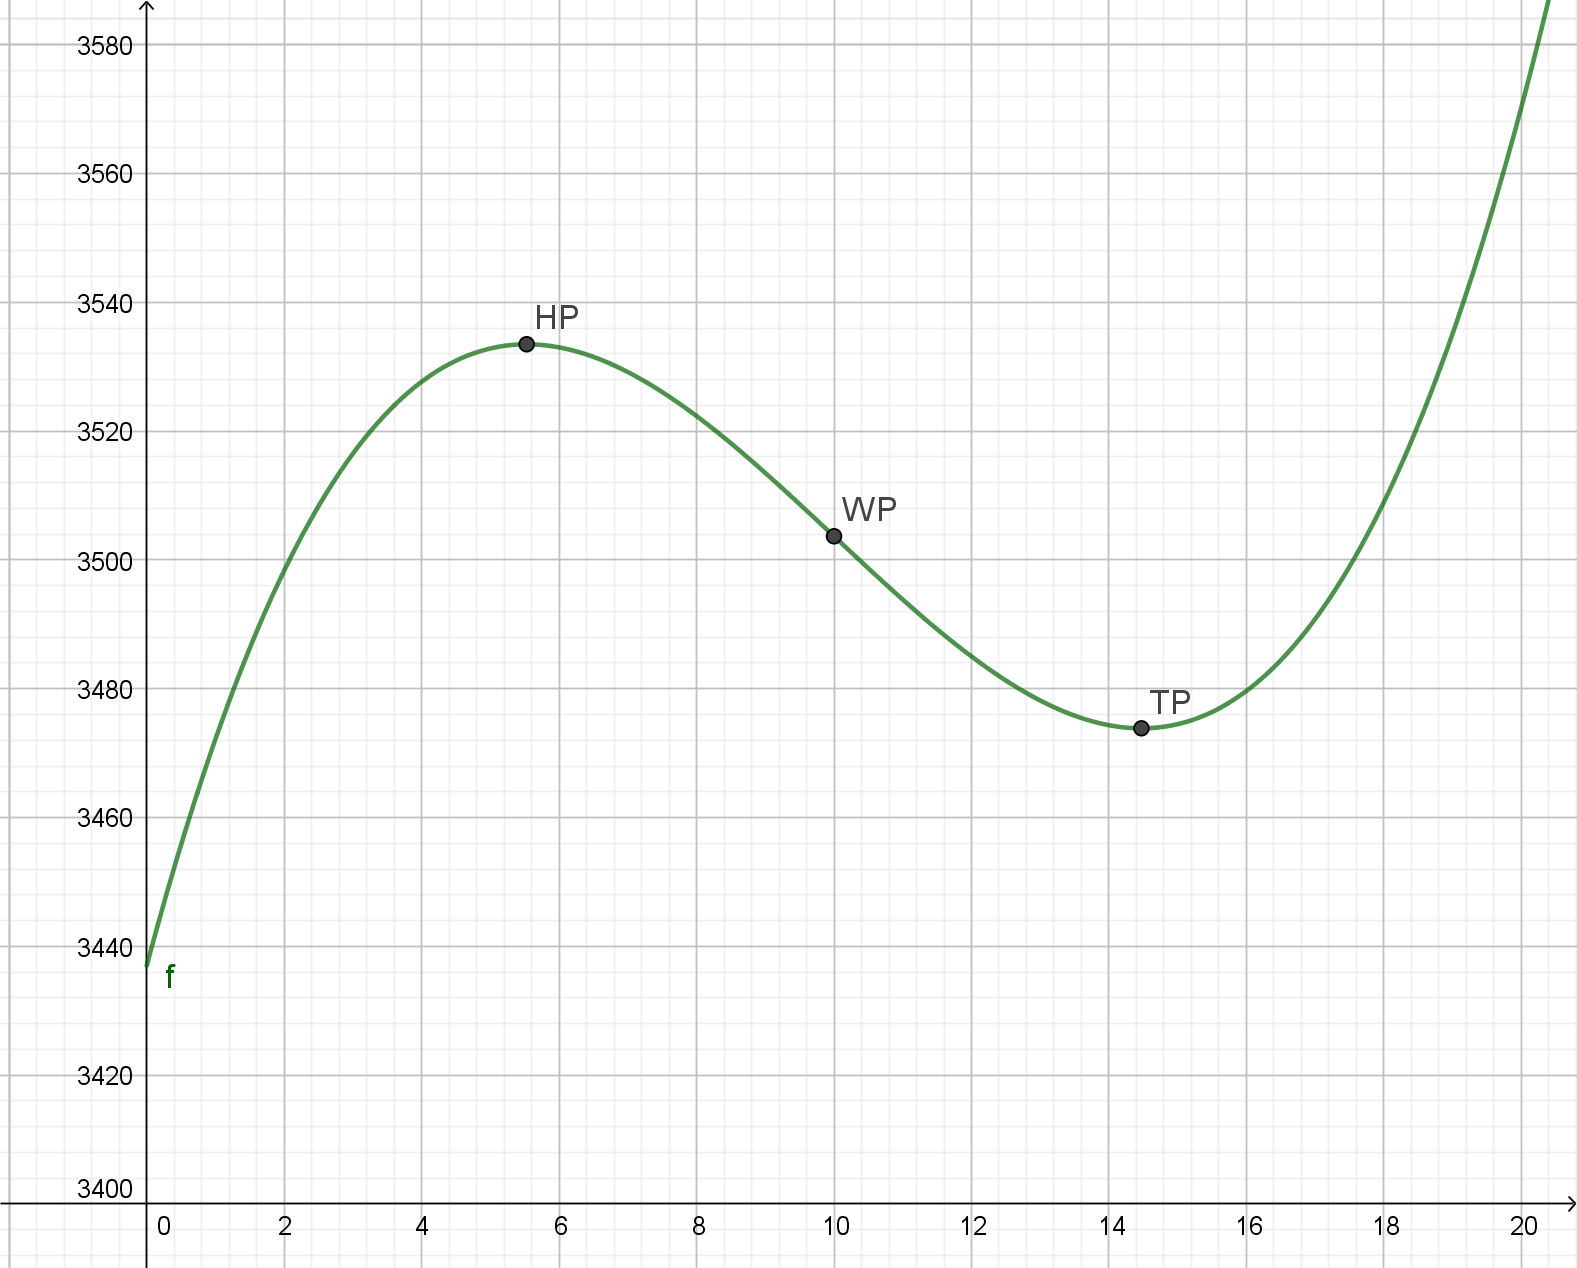
\includegraphics[width=0.95\textwidth]{../99_Bilder/LSG1.png}
			\end{center}
		\end{framed}
		\newpage
		\begin{framed}
			\noindent
			Die Zombieapokalypse ist ausgebrochen. Die Entwicklung der Infizierten kann mit \[f(x) = -x^4 + 12x^3\] modelliert werden.\\
			Dabei gibt \(x\) die vergangenen Tage an. Der Beginn des Ausbruchs entspricht also \(x = 0\) und \(y\) gibt die infizierten Personen in Tausend an.\\
			Es wird vermutet, dass nach dem Ausbruch entsprechende Gegenmaßnahmen gestartet wurden.
		\end{framed}
		\begin{itemize}
			\item[(a)] Bestimmen Sie Hoch-, Tief und Sattelpunkte, falls vorhanden!
		\end{itemize}
		\begin{framed}
			\noindent
			Zur Bestimmung der Hoch-, Tief- und Sattelpunkte benötigen wir zunächst die \underline{erste Ableitung und zweite Ableitung}!\\
			\par\noindent
			\(f'(x) = -4x^3+36x^2\)\\
			\(f''(x) = -12x^2 + 72x\)\\
			\par\noindent
			Wir bestimmen nun die \textbf{Nullstellen der ersten Ableitung} - also \(f'(x) = 0\).
			\begin{tabularx}{\textwidth}{ll}
				\(f'(x) = 0\)\\
				\(-4x^3 + 36x^2 = 0\) & |\(x^2\) ausklammern\\
				\(x^2(-4x + 36) = 0\)\\
			\end{tabularx}\\
			\par\noindent
			\textit{Ein Produkt \(a\cdot{}b = 0\), wenn einer der Faktoren a oder b Null ist.}\\
			\par\noindent
			\begin{tabularx}{\textwidth}{ll}
				\(\Rightarrow\) \colorbox{green!5}{\( x_1 = 0\)}\\
				\(\Rightarrow -4x +36 = 0\)\\
				\\
				\(-4x+36 = 0\) & |\(+4x\)\\
				\(36 = 4x\) & |\(:4\)\\
				\(x = 9\) & \(\Rightarrow\) \colorbox{green!5}{\(x_2 = 9\)}\\
			\end{tabularx}\\
			\par\noindent
			Bleibt zu bestimmen, ob es sich bei \(x_1, x_2\) um Hoch-, Tief- oder Sattelpunkte handelt. Hierfür betrachten wir \(f''(x_1)\) bzw. \(f''(x_2)\).
			\begin{tabularx}{\textwidth}{XX}
				\(f''(x_1) = -12\cdot{}0 + 72\cdot{}0 = 0\) & \(f''(x_2) = -12\cdot{}9 + 72\cdot{}9 = 540 > 0\)\\
				\(\Rightarrow\) \colorbox{green!5}{\(x_1\) ist ein Sattelpunkt} & \(\Rightarrow\) \colorbox{green!5}{\(x_2\) ist ein Tiefpunkt}
			\end{tabularx}\\
			\par\noindent
			Nun müssen wir nur noch die dazugehörigen Punkte berechnen.\\
			\begin{tabularx}{\textwidth}{XX}
				\(f(x_1) = -0^4 + 12\cdot{}0^3 = 0\) & \(f(x_2) = -9^4 + 12\cdot{}9^3 = 2187\)\\
				\(\Rightarrow\) \colorbox{green!10}{\(SP(0|0)\)} & \(\Rightarrow\) \colorbox{green!10}{\(TIP(9|2187)\)}
			\end{tabularx}
		\end{framed}
		\begin{itemize}
			\item[(b)] Bestimmen Sie den/die Wendepunkt/e und interpretieren Sie diesen/diese in Bezug auf die Situation!
		\end{itemize}
		\begin{framed}
			Für den Wendepunkt müssen wir die \textbf{Nullstelle der zweiten Ableitung} bestimmen.
			\begin{tabularx}{\textwidth}{ll}
				\(f''(x) = 0\)\\
				\(-12x^2 +72x = 0\) & | \(x\) ausklammern\\
				\(x(-12x+72) = 0\)
			\end{tabularx}\\
			\par\noindent
			\textit{Ein Produkt \(a\cdot{}b = 0\), wenn einer der Faktoren a oder b Null ist.}\\
			\par\noindent
			\begin{tabularx}{\textwidth}{ll}
				\(\Rightarrow\) \colorbox{green!5}{\(x_3 = 0 = x_1\)}\\
				\(\Rightarrow -12x+72 = 0\)\\
				\\
				\(-12x+72 = 0\) & |\(+12x\)\\
				\(72 = 12x\) & |\(:12\)\\
				\(x=6\) & \(\Rightarrow\) \colorbox{green!5}{\(x_4 = 6\)}
			\end{tabularx}\\
			\par\noindent
			Nun benötigen wir nur noch die Koordinaten zu den Wendepunkten.\\
			\par\noindent
			\begin{tabularx}{\textwidth}{XX}
				Da \(x_3 = x_1 \Rightarrow WP = SP\) & \(f(x_4) = -6^4 + 12\cdot{}6^3 = 1296\)\\
				\(\Rightarrow\) \colorbox{green!10}{\(WP_1(0|0)\)} & \(\Rightarrow\) \colorbox{green!10}{\(WP_2(6|1296)\)}
			\end{tabularx}\\
			\par\bigskip\noindent
			Zu Beginn des Ausbruchs, also bei \(x = 0\) ändert sich die Infektionsdynamik. Ab diesem Zeitpunkt nimmt die Anzahl der Neu-Infizierten rapide zu.\\
			Nach \(x=6\) Tagen haben die Gegenmaßnahmen eine Wirkung gezeigt und die Anzahl der Neu-Infizierten lässt nach. 
		\end{framed}
		\newpage
		\begin{itemize}
			\item[(c)] Skizzieren Sie einen Funktionsgraph auf Basis ihrer gewonnen Daten.
		\end{itemize}
		\begin{framed}
			\begin{center}
				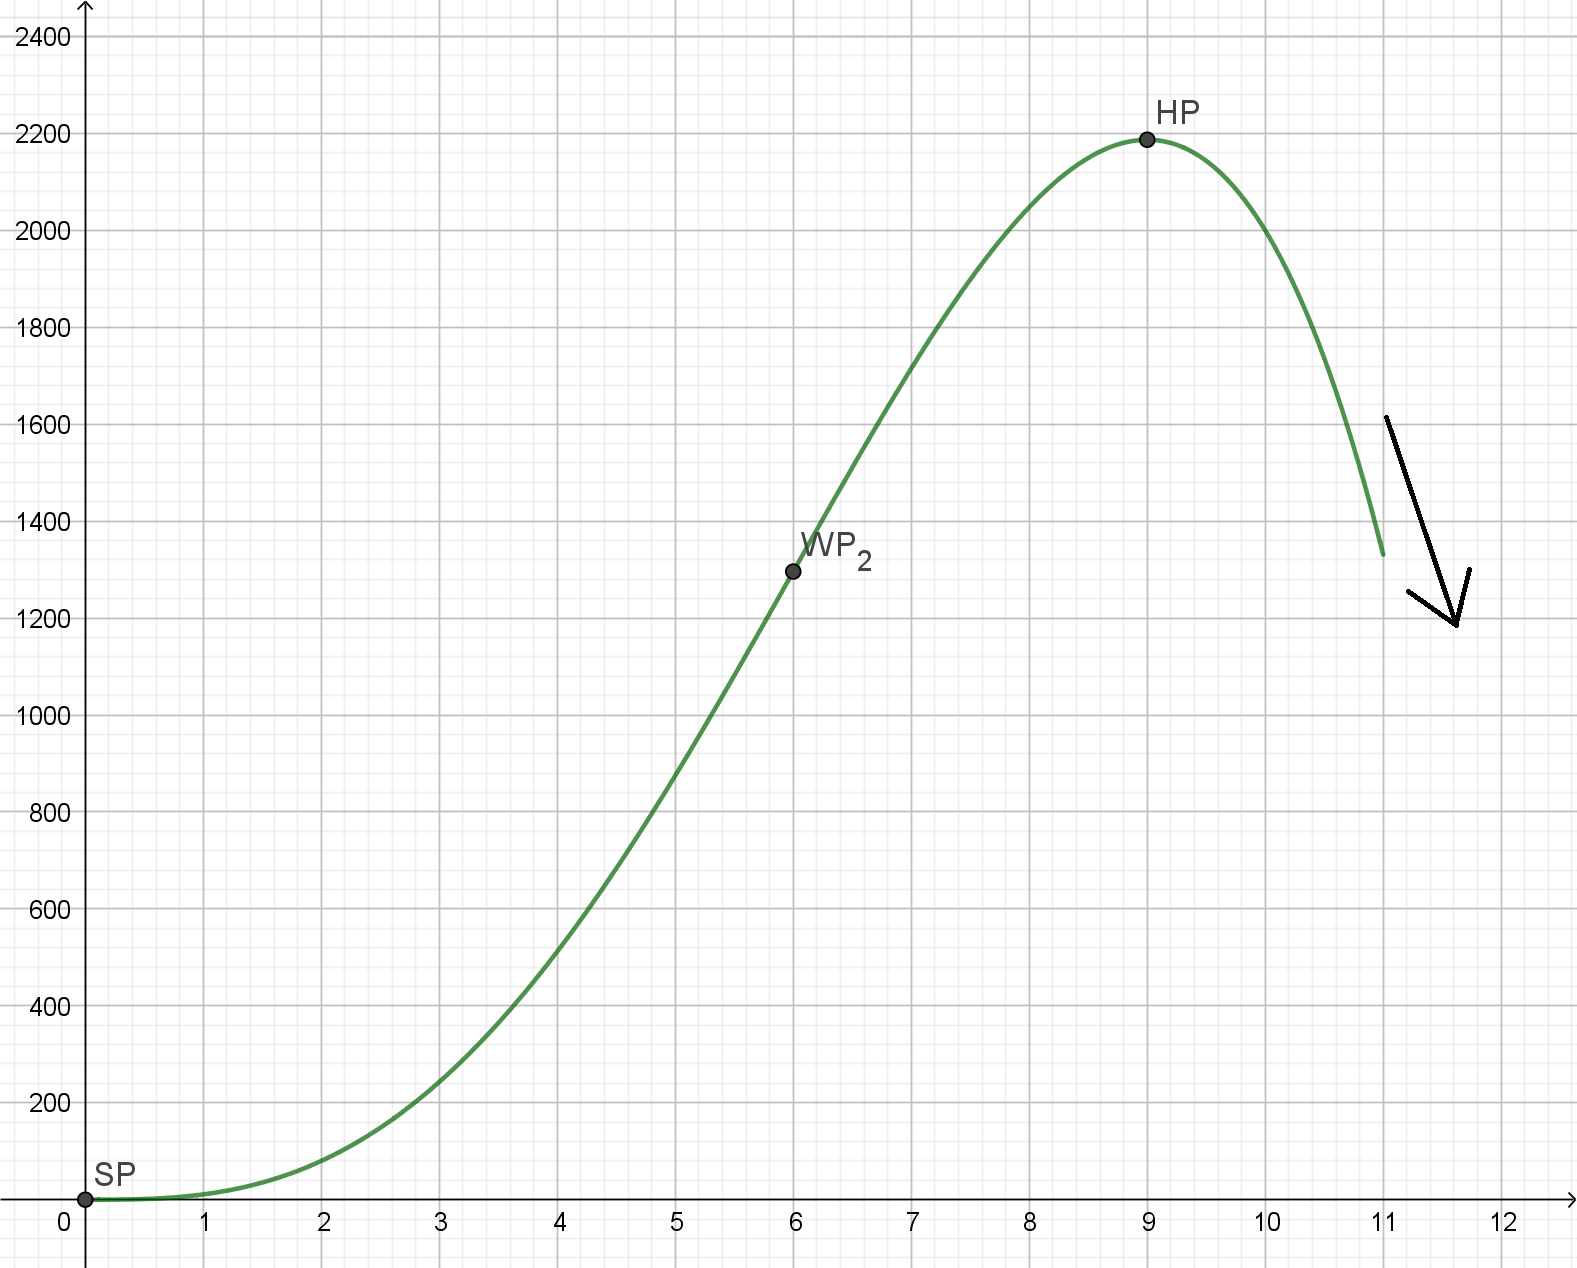
\includegraphics[width=\textwidth]{../99_Bilder/LSG2.png}
			\end{center}
		\end{framed}
		\begin{itemize}
			\item[(d)] Wird keine Gegenmaßnahme eingeleitet, würde sich die Infektionsdynamik ab Tag \(x = 6\) nicht mehr ändern. Bestimmen Sie die Infektionsdynamik an besagter Stelle und bestimmen Sie zudem die Anzahl der Infizierten nach 12 Tagen.
		\end{itemize}
		\begin{framed}
			\noindent
			Was bedeutet eigentlich, die Infektionsdynamik ändert sich nicht mehr?\\
			\par\noindent
			Im Prinzip sagt das nur aus, dass der Zuwachs, also die Anzahl Neu-Infektion, ab Tag 6 konstant bleiben. Wir bestimmen also die \textbf{Infektionsdynamik zum Zeitpunkt \(x=6\)} und erzeugen daraus eine \textbf{Geradengleichung durch den Punkt \(WP(6|1296)\)}.\\
			Anschließend kümmern wir uns dann um die Anzahl der Infektionen nach 12 Tagen. Aber eins nach dem anderen!\\
			\par\noindent
			Um die Infektionsdynamik zum Zeitpunkt \(x=6\) zu bestimmen, berechnen wir \(f'(6)\).\\
			\par
			\(f'(6) = -4\cdot{}6^3 +36\cdot{}6^2 = 432\)\\
			\par\noindent
			Unsere Gerade hat also die Steigung \(m=432\) und verläuft durch \(WP(6|1296)\). Mit dem Dreisatz folgt dann \(g(x) = 432x-1296\).\\
			\par\noindent
			Bleibt noch die Anzahl der Infizierten nach \(x=12\) Tagen zu bestimmen. Hierfür berechnen wir \underline{\(g(12) = 432\cdot{}12 -1296 = 3888\)}.\\
			\par\noindent
			Nach 12 Tagen sind es also \colorbox{green!10}{3888 Infizierte}.
		\end{framed}
		\rule{\textwidth}{0.1pt}
		\begin{framed}
			\noindent
			Bei einer ausgebrochenen Grippewelle kann die Entwicklung der Anzahl der Erkrankten mit \(f(x) = -\frac{1}{3}x^3 + 3x^2\) modelliert werden.\\
			Wie gewohnt entspricht \(x = 0\) dem Beginn der Grippewelle und \(y\) gibt die Anzahl der Erkrankten in Tausend an.
		\end{framed}
		\begin{itemize}
			\item[(a)] Führen Sie eine klassische Kurvendiskussion durch und skizzieren Sie den Funktionsgraphen in ein entsprechendes Koordinatensystem.\\
			Markieren Sie die charakteristischen Stellen des Funktionsgraphen!
		\end{itemize}
		\begin{framed}
			\noindent
			Nachfolgend führen wir eine klassischen Kurvendiskussion durch.\\
			\par\noindent
			\textbf{Definitions- und Wertebereich}\\
			\(\mathbb{D} = \{\mathbb{R}\}\)\\
			\(\mathbb{W} = \{\mathbb{R}\}\)\\
			\textbf{Ableitungen}\\
			\(f'(x) = -x^2 + 6x\)\\
			\(f''(x) = -2x + 6\)\\
			\(f'''(x) = -2\)\\
			\textbf{Symmetrie}\\
			Da \(f(x)\) sowohl gerade wie auch ungerade Exponenten beinhaltet, ist der Graph \colorbox{green!10}{nicht symmetrisch}.
			\textbf{Verhalten für große x-Werte}\\
			Hierfür benötigen wir nur den \textbf{charakteristischen Term} \(-\frac{1}{3}x^3\).\\
			\begin{tabularx}{\textwidth}{XX}
				\multicolumn{2}{l}{\(a = -\frac{1}{3}\) negativ, \(n = 3\) ungerade}\\
				\\
				\(f(x)\xrightarrow{x\rightarrow-\infty}\infty\) & \(f(x)\xrightarrow{x\rightarrow\infty}-\infty\)
			\end{tabularx}
			\textbf{Nullstellen}\\
			Wir berechnen \(f(x) = 0\).\\
			\par
			\begin{tabularx}{\textwidth}{ll}
				\(-\frac{1}{3}x^3 +3x^2 = 0\) & |\(x^2\) ausklammern\\
				\(x^2(-\frac{1}{3}x +3) = 0\)\\
				\\
				\multicolumn{2}{l}{Ein Produkt \(a\cdot{}b = 0\), wenn einer der Faktoren Null ist.}\\
				\\
				\(x^2 = 0\) & \(\Rightarrow x_{1,2} = 0\)\\
				\(-\frac{1}{3}x + 3 = 0\) & |\(+\frac{1}{3}x\)\\
				\(3 = \frac{1}{3}x\) & |\(\cdot{}3\)\\
				\(x = 9\) & \(\Rightarrow x_3 = 9\)
			\end{tabularx}
			Unsere Funktion \(f(x)\) hat bei \colorbox{green!10}{\(x_{1,2}=0\)} eine doppelte Nullstelle und bei \colorbox{green!10}{\(x_3 = 9\)} eine einfache Nullstelle.\\
			Die dazugehörigen Punkte sind \underline{\(N_1 (0|0), N_2(0|0)\)} und \underline{\(N_3(9|0)\)}.\\
			\par\noindent
			\textbf{Extremstellen}\\
			Wir berechnen \(f'(x) = 0\)\\
			\begin{tabularx}{\textwidth}{ll}
				\(-x^2+6x = 0\) & |\(x\) ausklammern\\
				\(x(-x+6) = 0\)\\
				\\
			\end{tabularx}
			Ein Produkt \(a\cdot{}b = 0\), wenn einer der Faktoren Null ist.\\
			\begin{tabularx}{\textwidth}{ll}
				\\
				\(x = 0\) & \(\Rightarrow x_4=0\)\\
				\(-x+6 = 0\) & |\(+x\)\\
				\(6 = x\) & \(\Rightarrow x_5=6\)\\
			\end{tabularx}
			Unsere Extrempunkte liegen bei \colorbox{green!5}{\(x_4=0\)} und bei \colorbox{green!5}{\(x_5=6\)}.\\
			Jetzt müssen wir bestimmen, ob es sich um HOP bzw. TIP handelt.\\
			Dafür bestimmen wir \(f''(x_4)\) bzw. \(f''(x_5)\).\\
			\begin{tabularx}{\textwidth}{ll}
				\\
				\(f''(x_4) = -2\cdot{}0 +6 = 6 > 0\) & \(\Rightarrow x_4\ \text{ist}\ TIP\).
			\end{tabularx}
			Da \(x_4 = x_{1,2}\) kennen wir die Koordinaten \colorbox{green!10}{\(TIP(0|0)\)}.\\
			\begin{tabularx}{\textwidth}{ll}
				\\
				\(f''(x_5) = -2\cdot{}6 +6 = -6 < 0\) & \(\Rightarrow x_5\ \text{ist}\ HOP\).\\
			\end{tabularx}
			Auch hier bestimmen wir direkt die Punkt-Koordinaten.\\
			\begin{tabularx}{\textwidth}{ll}
				\\
				\(f(x_5) = -\frac{1}{3}\cdot{}6^3 +3\cdot{}6^2 = 36\)\\
				\(\Rightarrow\) \colorbox{green!10}{\(HOP(6|36)\)}
			\end{tabularx}\\
			\par\noindent
			\textbf{Wendestelle}\\
			Wir berechnen \(f''(x) = 0\).\\
			\begin{tabularx}{\textwidth}{ll}
				\(-2x+6 = 0\) & |\(+2x\)\\
				\(6 = 2x\) & |\(:2\)\\
				\(x = 3\) & \(\Rightarrow x_6=3\)\\
			\end{tabularx}
			Unsere Funktion hat also einen Wendepunkt an der Stelle \colorbox{green!10}{\(x_6=3\)}.\\
			Den dazugehörigen Punkt bestimmen wir wie folgt.\\
			\begin{tabularx}{\textwidth}{ll}
				\\
				\((f(x_6) = -\frac{1}{3}\cdot{}3^3 +3\cdot{}3^2 = 18\)\\
				\(\Rightarrow\) \colorbox{green!10}{\(WP(3|18)\)}.\\
			\end{tabularx}\\
			\par\noindent
			\textbf{Krümmungsverhalten}\\
			Für das Krümmungsverhalten betrachten wir die \underline{Monotonie der ersten Ableitung} auf den Intervallen \(I_1 = \left(-\infty,x_W\right)\) bzw. \(I_2 = \left(x_W,\infty\right)\).\\
			\par\noindent
			\begin{tabularx}{\textwidth}{X|X}
				\(I_1 = \left(-\infty,x_W\right)\) & \(I_2 = \left(x_W,\infty\right)\)\\
				Für alle \(x_0,x_1 \in I_1\) mit \(x_0 < x_1\) gilt \(f'(x_0) < f'(x_1)\) & Für alle \(x_0,x_1 \in I_1\) mit \(x_0 < x_1\) gilt \(f'(x_0) > f'(x_1)\)\\
				\(\Rightarrow\) \colorbox{green!10}{\(f(x)\) ist \underline{linksgekrümmt}} & \(\Rightarrow\) \colorbox{green!10}{\(f(x)\) ist \underline{rechtsgekrümmt}}
			\end{tabularx}\\
			\par\noindent
			Wir haben alle notwendigen Informationen, um den Graph zur gegebenen Funktion skizzieren zu können. Man überträgt also die charakteristischen Punkte in das Koordinatensystem und verbindet die Punkte entsprechend dem Krümmungsverhalten.\\
			\begin{center}
				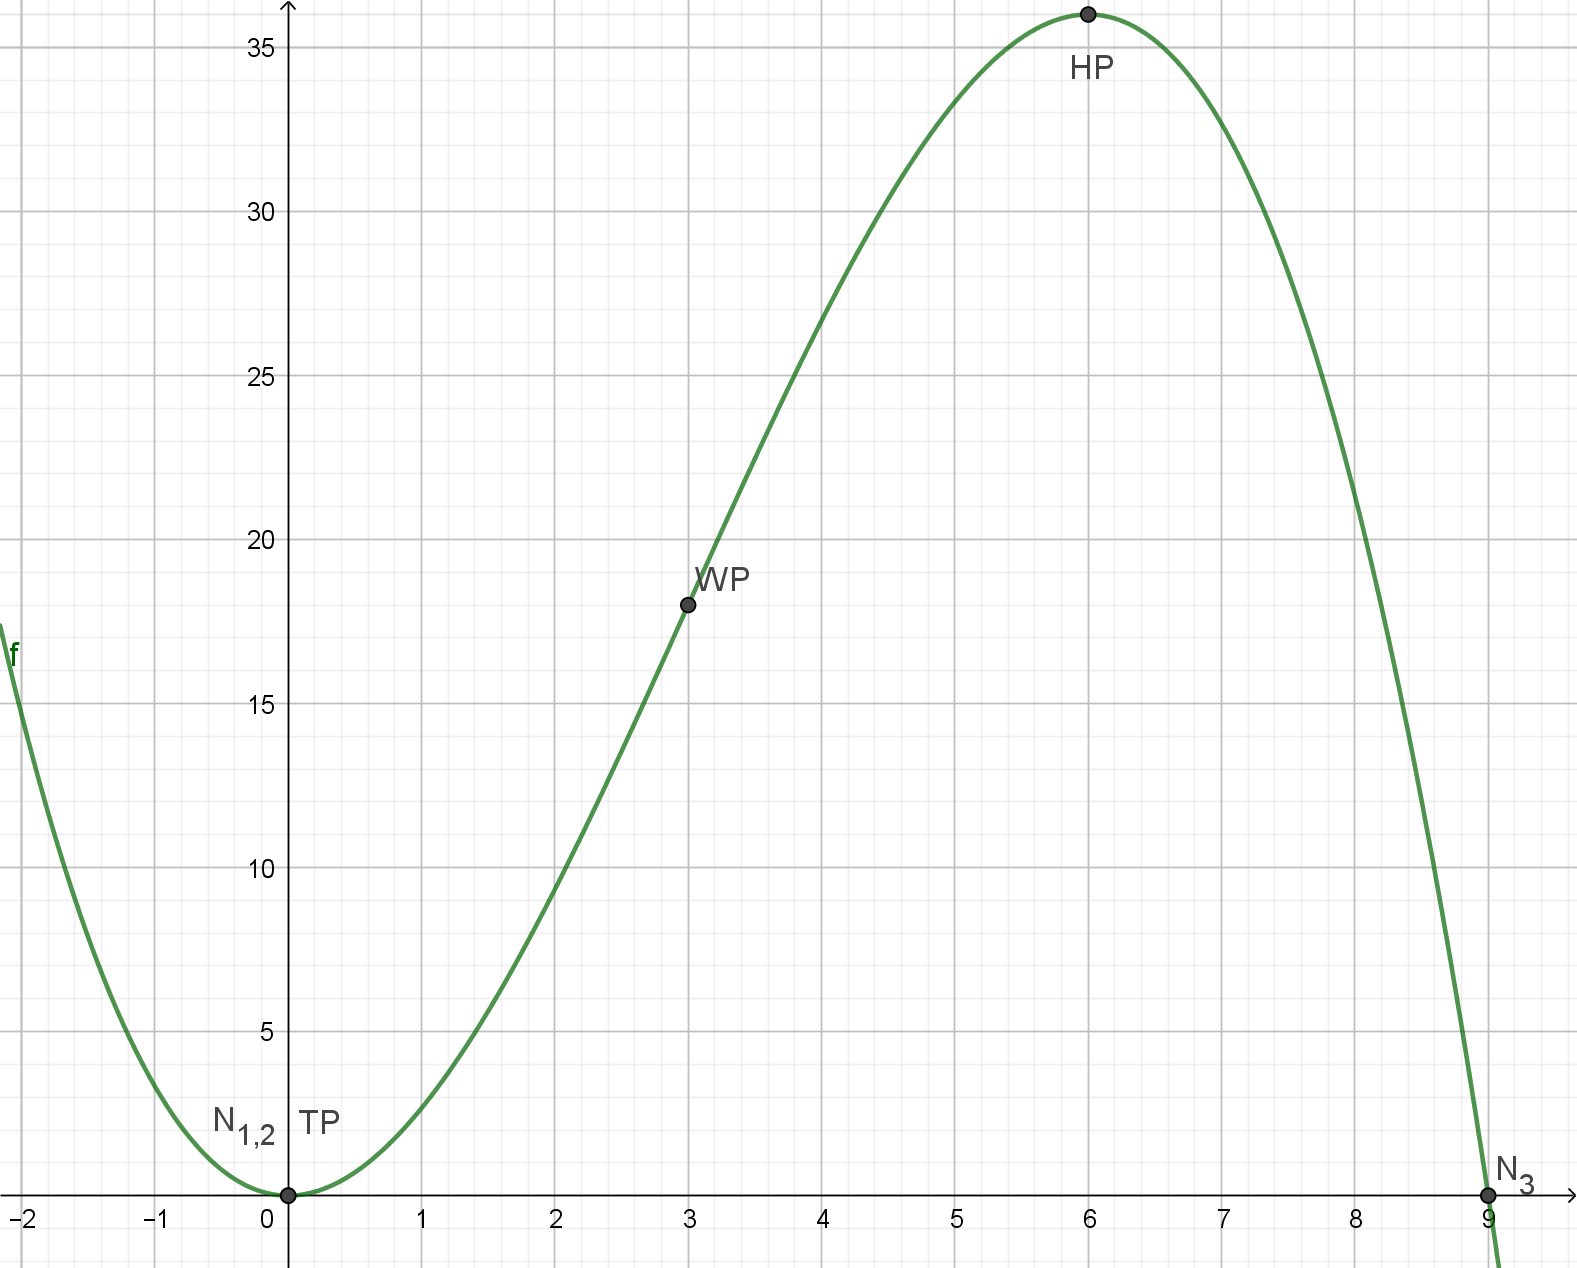
\includegraphics[width=\textwidth]{../99_Bilder/LSG3.png}
			\end{center}
		\end{framed}
		\begin{itemize}
			\item[(b)] Es kann zu verschieden intensiven Ausbrüchen kommen. Diese werden durch einen Parameter in das Modell integriert. Die dazugehörige Funktionsgleichung lautet also:
			\[f(x) = -\frac{1}{3}x^3 +tx^2\]
			Bestimmen Sie die Extrem- und Wendestelle(n) in Abhängigkeit von \(t\).\\
			Beschreiben Sie zusätzlich den Einfluss des Parameters auf die Entwicklung der Anzahl der Erkrankten.
		\end{itemize}
		\begin{framed}
			\noindent
			Wie in Teilaufgabe (a) bestimmen wir die Extrem- bzw. Wendestellen mit der ersten bzw. zweiten Ableitung. Da unsere Funktion diesmal einen Parameter \(t\) enthält, benötigen wir die Ableitungen für ebendiese.\\
			\(f'(x) = -x^2 +2tx\)\\
			\(f''(x) = -2x +2t\)\\
			\par\noindent
			\begin{tabularx}{\textwidth}{Xl|Xl}
				\textbf{Extremstelle} \(f'(x) = 0\) & & \textbf{Wendestelle} \(f''(x) = 0\)\\
				\(-x^2 + 2tx = 0\) & |\(x\) ausklammern & \(-2x + 2t = 0\) & |\(+2x\)\\
				\(x(-x+2t) = 0\) & & \(2t = 2x\) & |\(:2\)\\
				\(\Rightarrow x_{E_1} = 0\) & & \(\Rightarrow\) \colorbox{green!10}{\(x_W = t\)}\\
				\(-x+2t = 0\) & |\(+x\)\\
				\(\Rightarrow\) \colorbox{green!10}{\(x_{E_2} = 2t\)}
			\end{tabularx}\\
			\par\noindent
			Je größer der Parameter \(t\), desto später im Zeitverlauf wird das Maximum der Erkrankten erreicht. Zudem wird, je größer der Parameter \(t\) ist, stagniert die Anzahl der Neuerkrankungen später.
		\end{framed}
	\end{worksheet}
\end{document}